\section{Our Approach}
\label{integriscreen:sec:systemDesign}

We start by providing the general idea of visual supervision of user input; then discuss challenges to be addressed successfully to ensure that interactions with the remote server match user's intentions.


\subsection{Approach Overview}
\label{integriscreen:sec:systemDesign:overallApproach}


\begin{figure}[t]
	\centering
	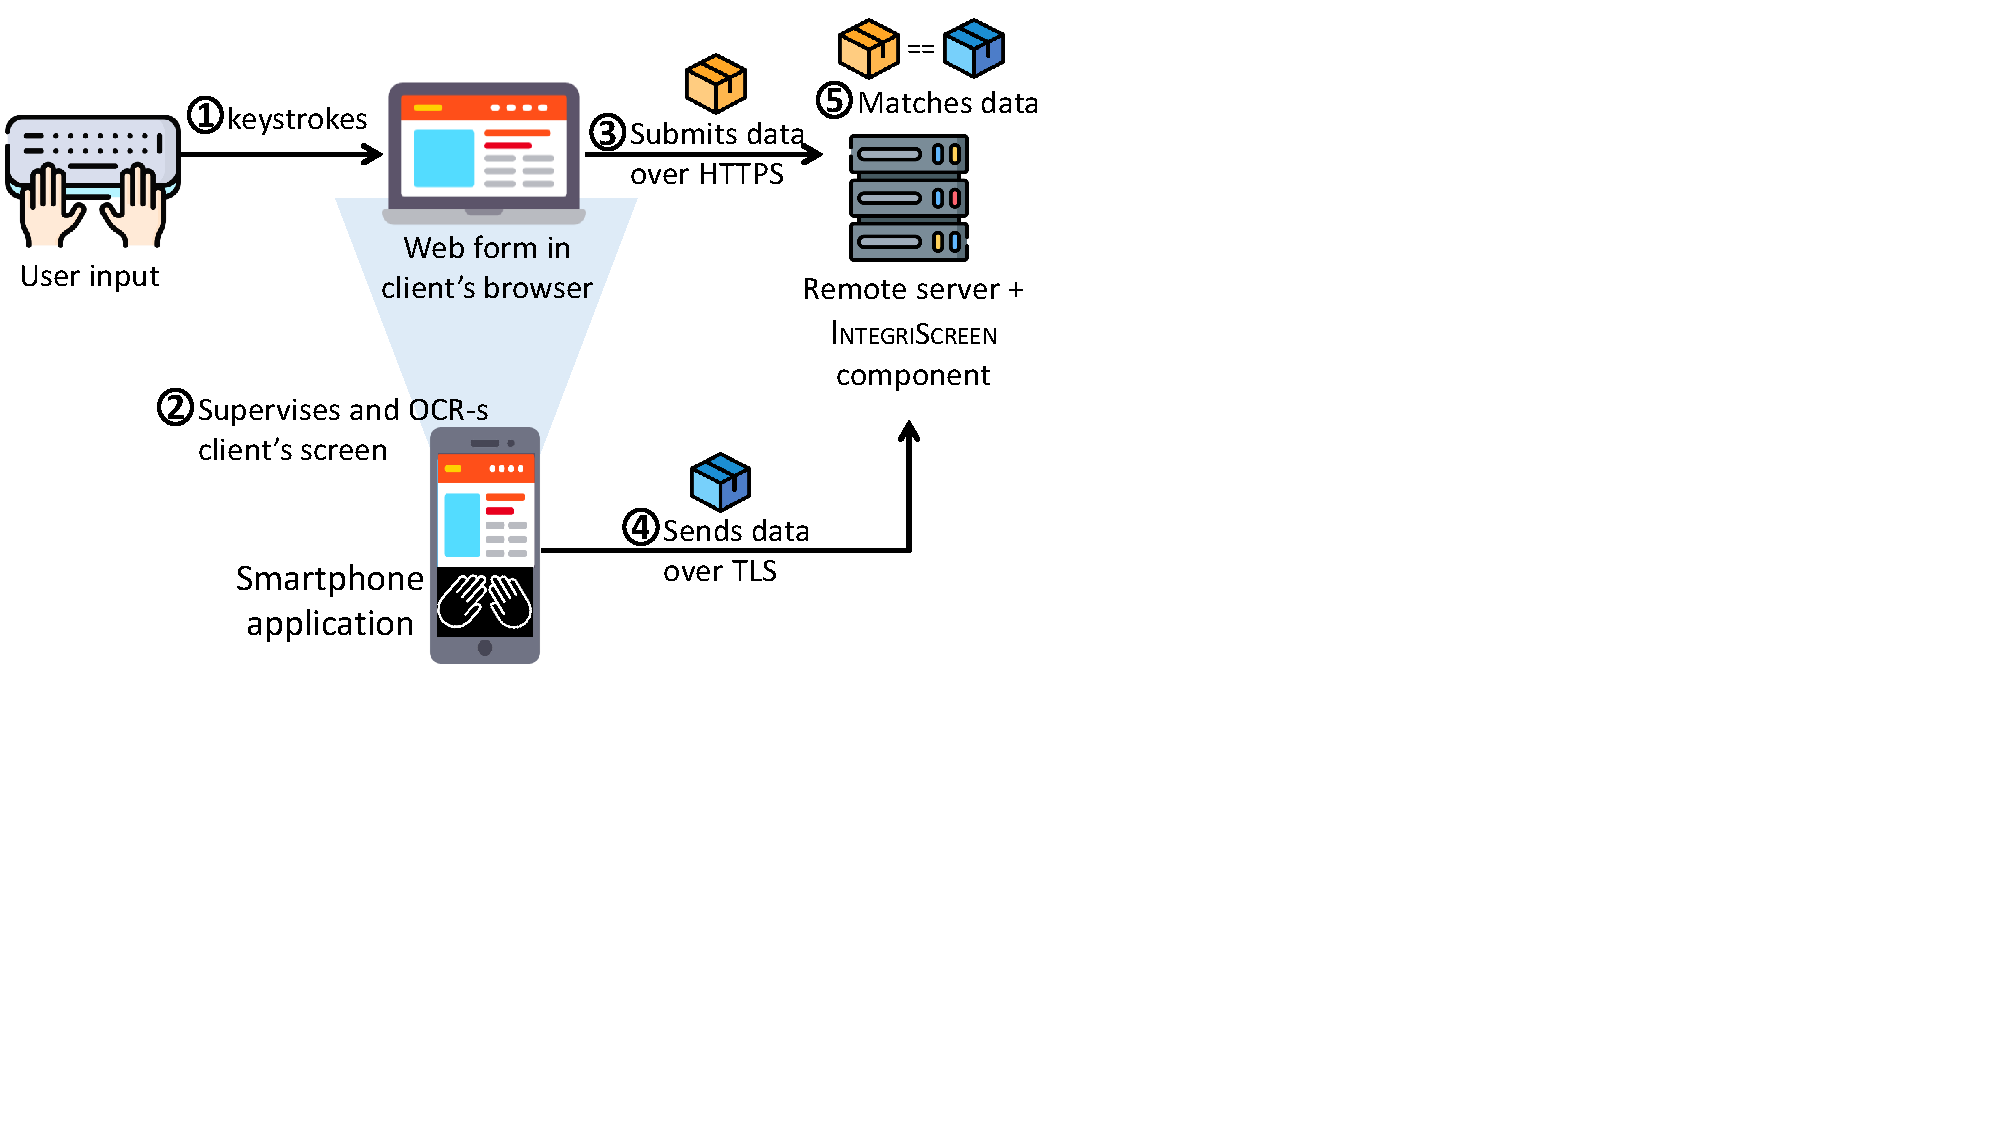
\includegraphics[trim={0 7cm 17cm 0},clip,width=0.75\linewidth]{chapters/IntegriScreen/img/systemModel.pdf}
	\caption[\sysname overview.]{\textbf{\sysname overview.}
	    \one The user inputs data into a web form on an untrusted host, \two while the smartphone's camera captures the interaction.
	    \three Data is submitted both from the host and \four from the \app.
		\five The server checks authenticity of the received data by comparing the two channels.}
	\label{integriscreen:fig:systemModel}
\end{figure}


The system consists of 3 main components: (i) the web form and its code, running on an untrusted local host; (ii) the trusted remote \server with an \name web server component; and (iii) the mobile app, running on the smartphone under user's control.

An overview of our approach is depicted in Figure~\ref{integriscreen:fig:systemModel} and described below:

\begin{enumerate}
  \item[\one] The user inputs the data through the form running in the untrusted host's browser.

  \item[\two] The \app extracts the data input by the user by performing optical character recognition (OCR) of the host screen to generate a visual \POI.

  \item[\three] The browser transfers the user's input over a \https channel to the remote server.

  \item[\four] The \app then transfers the generated \POI to the remote server over a dedicated \tls channel between the smartphone and the remote server.

  \item[\five] Upon receiving data from both the browser and the mobile device, the \name server component matches the data from two inputs, as shown in Figure~\ref{fig:traceMatching}.
  If the two inputs match exactly, the web server accepts the input; otherwise, it rejects it.
\end{enumerate}



\begin{figure}[t]
    \centering
    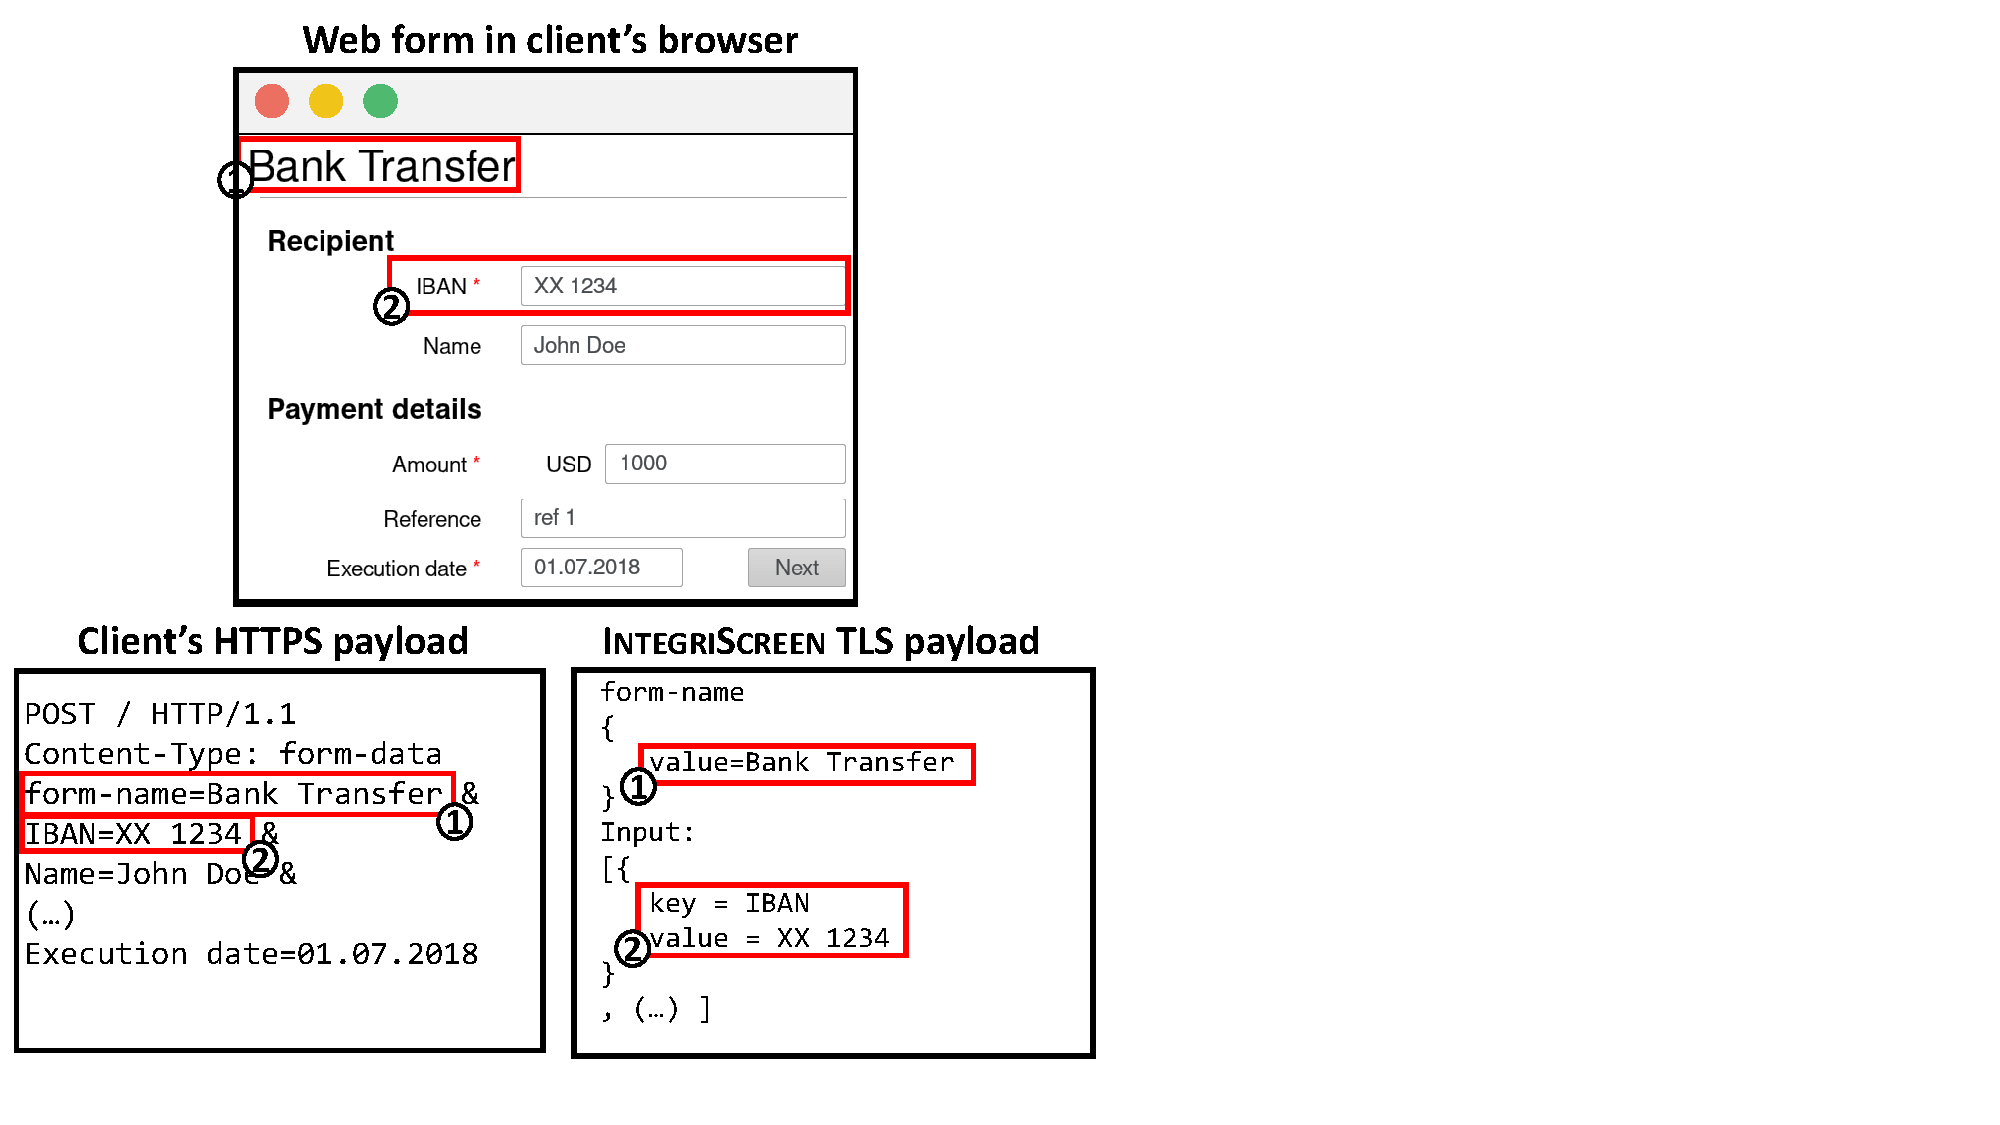
\includegraphics[trim={0 1cm 14cm 0},clip,width=0.7\linewidth]{chapters/IntegriScreen/img/inputMatching.pdf}
\caption[\sysname input data matching.]{\textbf{\sysname input data matching.}
        The server receives data (e.g., \one and \two) from two channels: (i) the \https channel from the host, and (ii) the TLS channel from the \name mobile app.}
    \label{fig:traceMatching}
    \vspace{0.3cm}
\end{figure}



% \myparagraph{Security of the approach}
The design of \sysname protects against the majority of attacks discussed in Section~\ref{sec:intro}.
Even after compromising the host and obtaining the victim's authentication credentials, the adversary can neither generate new requests nor covertly modify the data before submitting.
This is prevented by the server, which would reject the requests due to not receiving a matching \POI.


\subsection{Challenges}
\label{integriscreen:sec:systemDesign:challenger}

There remain several other challenges and possible attacks to be addressed to ensure that all received requests truly correspond with the user's intended input, presented in the following.

\myparagraph{Preventing UI manipulation attacks}
With our initial design, the adversary is prevented from modifying the data in transit between the user and the server.
However, he fully controls the host device operations, including loading and presenting the user interface: by modifying elements of the user interface, the adversary can trick the user into entering the \textit{wrong} values -- by changing the semantics of the input.
For example, in case of remote configuration of medical devices, changing a single text label in the user interface (or even only its relative position!) can result in an anesthesiologist entering a value using a wrong measurement unit, e.g. ml instead of dl, and seriously harming the patient due to a tenfold increase in the drug dosage.
These attacks would be successful even if the user re-types his inputs into a special device that generates a TAN (transaction authorization number) code.

As we discuss in Section~\ref{sec:hardenUI}, \sysname prevents such attacks by requiring that the remote server provides a specification of the user interface (UI) and by ensuring that the UI is loaded on the host's screen matches its specification during all stages of user input.


\myparagraph{Preventing on-screen data modification attacks}
So far, there was no explicit discussion of the moment at which the mobile app captures the data shown on the screen.
Even if the data shown on the host's screen is truthfully sent to the remote server, user input integrity is not necessarily guaranteed if data extraction happens only before the form is submitted from the host.
Despite the user entering the intended data, the adversary can subsequently modify the screen's content so that the user does not notice the change, the \app records it, and the server thus receives the same maliciously modified data from both channels.

For example, in the web form shown in Figure~\ref{fig:traceMatching}, while the user is focused on entering the payment amount or execution date, the adversary could modify the IBAN field without the user noticing.
Furthermore, the adversary could modify the values shown on the screen. At the same time, the user is absent, not focused on the screen, or a malicious window temporarily overlays the browser form to shift the victim's attention.

As we discuss in Section~\ref{sec:hardenUI}, a crucial step to generate \PsOI\ is real-time, continuous supervision of the screen content, with specific expectations about the design and behavior of the user interface, and only allowing the mobile app's \POI to be submitted if the data has been generated in accordance to these rules.




\myparagraph{Challenges of visually supervising another device}
Computers still struggle in understanding visual computer interfaces.
For example, even a seemingly straightforward task of detecting computer screens in images is still an open research question~\cite{detectingScreens}.
It is, therefore, an interesting challenge to propose a system that requires \emph{minimal changes to the user interface}, while at the same time achieving security guarantees against the adversarial host system.

Furthermore, despite recent significant improvements in Optical Character Recognition (OCR) based on deep learning~\cite{tesseractOCR}, achieving \emph{consistent continuous detection of textual content} on another device's screen requires several deliberate design choices.
Using OCR libraries naively, e.g. attempting to detect all text shown on a large part of the host's screen, results both in low performance ($<0.5$ fps) and significant parts of text not being detected due to different font sizes and types.

Finally, continuous visual supervision of another device's screen requires that the mobile device is statically positioned so that its camera captures the whole area of interest.
This, however, means that the supervised screen is captured from different positions and different angles and requires \emph{precise estimation and removal of the pose} between the two devices.


\subsection{Design Goals}
Successful user input supervision to extract user intent should:

\begin{enumerate}
	\item Authenticate remote requests that users make through compromised hosts, i.e., ensure that the adversary can neither generate nor modify existing remote requests successfully.

	\item Ensure that users are not being manipulated into entering and submitting data that they would not submit in the absence of the adversary.

	\item Require minimal added interaction in the absence of attacks: do not require that users input or explicitly verify any data except on the host device.
\end{enumerate}
